\begin{figure}[htbp]
\centering
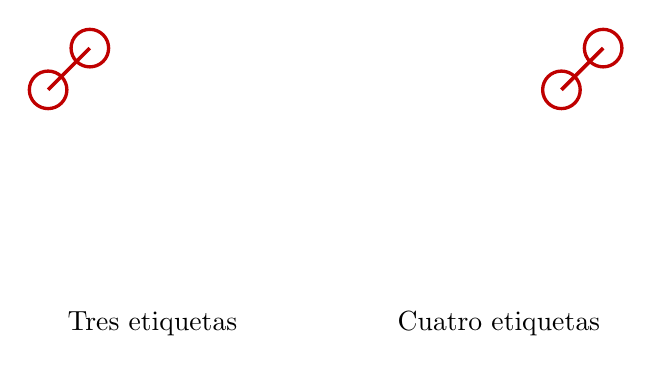
\begin{tikzpicture}[x=.53cm,y=.53cm]
 \foreach \tipo/\dx/\uno/\dos in {3/0/2/1,4/8.3/6/5}{
  \begin{scope}[shift={(\dx,0)}]
   \bcuadricula{6}
   \draw[red!75!black,line width=1.3pt] ({\uno-.5},5.5) -- ({\dos-.5},4.5);
   \bmarca{6}{1}{\uno}
   \bmarca{6}{2}{\dos}
   \draw[red!75!black,line width=1.2pt] ({\uno-.5},5.5) circle[radius=.45];
   \draw[red!75!black,line width=1.2pt] ({\dos-.5},4.5) circle[radius=.45];
   \foreach \rr/\cc in {1/2,2/4,3/6,4/1,5/3,6/5}{\breina{6}{\rr}{\cc}}
   \ifnum\tipo=3
    \node at (3,-1.1) {Tres etiquetas};
   \else
    \node at (3,-1.1) {Cuatro etiquetas};
   \fi
  \end{scope}
 }
\end{tikzpicture}
\caption{Dos testigos en el tablero de orden seis de la solución $\pi=(2,4,6,1,3,5)$. Las filas se
numeran desde uno de arriba abajo y las columnas desde uno de izquierda a derecha. Las coronas son las
reinas de $\pi$. Dos círculos unidos señalan las casillas $(i,\pi(j))$ e $(i',\pi(j'))$ que comparten
diagonal. A la izquierda, $(i,i',j,j')=(1,2,1,4)$ marca $(1,2)$ y $(2,1)$ y usa tres etiquetas
distintas. A la derecha, $(1,2,3,6)$ marca $(1,6)$ y $(2,5)$ y usa cuatro. Con sólo dos etiquetas se
tendría $\{i,i'\}=\{j,j'\}$ y $|i-i'|=|\pi(i)-\pi(i')|>0$, lo que haría que dos reinas de la solución
se atacasen.}\label{fig:testigos}
\end{figure}
